We apply our algorithm to several different settings:
\begin{itemize}
\item Logistic regression when the MLE exists.  The gradient $\nabla \ell(\beta)$ can be calculated exactly in this setting and thus our algorithm is guaranteed to converge.  We compare the results to those attained by \texttt{glm} function in R, which we treat as the truth.  Also, we compare the performance to stochastic approximation.  We choose a starting value for which Newton-Raphson fails.

\item Ising model, when the MLE exists.  The gradient $\nabla \ell(\beta)$ must be approximated in this setting via MCMC.  Although our algorithm is not guaranteed to converge in theory, it is still effective in practice.  We again compare the performance to stochastic approximation.

\item 9-node undirected ERGM with two-dimensional sufficient statistics.  Here we explore cases where MLE does and does not exist.  Our algorithm finds the MLE when
exists, and finds the LCM MLE and its support when it does not.  These can then
be used to constructed one-sided confidence intervals for the natural parameters.
\end{itemize}

\section{Example: logistic regression}
We illustrate the application of our algorithm in the case of a logistic regression 
with a starting point far from the 
solution.  In such a case, the Hessian matrix is often near-singular and algorithms 
such as Newton-Raphson which rely 
on it will fail.  For classical SA with step size $1/k$, the magnitudes of the updates 
diminishes too quickly for 
the parameter estimates to approach the MLE in a reasonable amount of time.

The response vector $Y$ has components that are Bernoulli trials with mean vector $p$.  
The natural parameter is $
\theta_i = \log \left( \frac{p_i}{1-p_i} \right )$, which is modeled componentwise as 
a linear function of the 
predictors $1, x_1, \ldots, x_{q}$, so that
\begin{align*}
	\theta_i &= \beta_0 + \beta_1 x_{1i} + \beta_2 x_{2i} + \cdots + \beta_{q} x_{q
\,i} = \beta^T x_i \qquad
i = 1, \ldots, n
\end{align*}
where $\beta = (\beta_0, \ldots, \beta_{q} )^T$ and $x_i = ( 1, x_{1i}, \ldots, x_{q 
i})^T$.  

Defining the model matrix $M$ to be the $n \times (q+1)$ matrix with the $x_i$ as 
rows, we can express $\theta = M \beta
$.  This in turn allows us to reparameterize the exponential family  as one with $
\beta$ as the natural parameter 
vector and $M^T y$ the vector of statistics with log likelihood
\begin{align*}
		 \ell(\beta) &=  \beta^T (M^T y) - c(\beta),
\end{align*}
where $y$ is the vector of observed Bernoulli responses.
By \eqref{E:nabla ell}, the gradient is
\begin{align*}
	\nabla \ell( \beta ) &=  M^T y - \E_{\beta}(M^T Y) = M^T( y - \E_{\beta}(Y) ),
\end{align*}
where $\E_{\beta}(Y) = \frac{1}{1 + \exp(-M \beta)}$ can be calculated exactly.  This 
allows us to directly apply 
Theorem~\ref{Thm:Line Search works}.

Suppose we specify our true parameter value to be $\beta = (0, 2, 2, 1, 1, 0, 0, 0)^T$ 
and use 100 independent draws 
from a correlated multivariate normal distribution centered at 0 as our predictors to 
generate 100 independent 
Bernoulli trials.  
Fitting these data using the R function \texttt{glm}, we find the MLE of $\beta$ to be
\begin{align*}
	\betaMLE = (  0.635,  5.949, 1.273, 0.180, 1.006, 1.536, -2.252, -0.472 )^T,
\end{align*}
where the disparity to the true value of $\beta$ results from a relatively small 
sample size of $n=100$.
We use $\beta_0 = ( 5, 4, 3, 2, 1, 0, -1, -2)^T$ for the starting point for our line 
search algorithm, a point for 
which Newton-Raphson fails due to a nearly singular Hessian matrix.  

We measure the performance of our algorithm in terms of the total number of iterations 
used, where each iteration 
requires the evaluation of the gradient, $\nabla \ell( \beta_k + \alpha_k p_k )$.  
Typically, several iterations take 
place in an inner loop to find a step size $\alpha_k$ that meets the curvature 
condition \eqref{E:curvature mod}, a 
process that grows increasingly difficult as the estimates near the MLE since the 
rightmost term in \eqref{E:curvature 
mod} gets smaller in magnitude.  Once an acceptable step size is found, the parameter 
estimate $\beta_k$ is updated and 
a new search direction is determined, requiring another evaluation of the gradient.

Our algorithm took 54 iterations over 20 different search directions to get $\lVert 
\nabla \ell( \beta_k ) \rVert < 
0.01$ and arrive at an estimate for the MLE that differs from the \texttt{glm} result 
by 0.0117 in Euclidean distance 
(See Table~\ref{Table:Logistic}).  
Using the Polak-Ribi\`{e}re conjugate gradient method described in the previous 
section  resulted in comparably sharp 
MLE estimates (see Table~\ref{Table:Logistic}) in fewer iterations---28 over 11 search 
directions---a noticeable 
improvement. 

We also applied  SA with step size $1/k$ (setting $A=1$, $B=0$ in \eqref{E:SA step 
size}) from the same starting point 
$\beta_0$.  The choice of constants $A$ and $B$ in the step size is of course not 
likely to be optimal;
however, we want to apply SA without trial and error experimentation.  
After 10,000 iterations, the parameter estimates look nothing at all like the MLE (See 
Table~\ref{Table:Logistic}).  
The starting point $\beta_0$ is so far from the MLE and the step sizes so small that 
the algorithm does not converge in a reasonable amount of time.
Table~\ref{Table:step size} shows the first 20 step sizes used by SA and our line 
search. Our line search continues to 
use step sizes of relatively large magnitude even well into the process.  It should be 
noted that these 20 step sizes 
correspond to the first 20 iterations of SA but all 54 iterations of our line search 
algorithm since it spends several 
iterations finding an acceptable step size for each update.


% latex table generated in R 2.10.1 by xtable 1.5-6 package
% Tue May  4 17:37:01 2010
\begin{table}
\caption{Comparison of MLEs of $\beta$ for Example 1: MLE = \texttt{glm}, Steep = line 
search using steepest ascent, 
CG = line search using conjugate gradient, and SA =  SA with step size = $1/k$, 
terminated at 10,000 iterations,
$n$ = number of iterations.  Our 
proposed algorithm arrives at nearly identical MLE estimates to \texttt{glm}.}
\begin{center}
\begin{tabular}{rrrrrrrrrr}
  \hline
 & $n$ & $\beta[1]$ & $\beta[2]$ & $\beta[3]$ & $\beta[4]$ & $\beta[5]$ & $\beta[6]$ & 
$\beta[7]$ & $\beta[8]$ \\ 
True $\beta$ & & 0.000 & 2.000 & 2.000 & 1.000 & 1.000 & 0.000 & 0.000 & 0.000 \\ 
  $\hat{\beta}_{\textrm{MLE}}$ & & 0.635 & 5.949 & 1.273 & 0.180 & 1.006 & 1.536 & 
$-2.252$ & $-0.472$ \\ 
  $\hat{\beta}_{\textrm{Steep}}$ & 54 & 0.633 & 5.938 & 1.272 & 0.181 & 1.005 & 1.535 
& $-2.249$ & $-0.470$ \\ 
  $\hat{\beta}_{\textrm{CG}}$ & 28 & 0.631 & 5.936 & 1.272 & 0.181 & 1.003 & 1.532 & 
$-2.244$ & $-0.470$ \\    
  $\hat{\beta}_{\textrm{SA}}$ & $10^4$ & 1.280 & 10.619 & 5.588 & 4.005 & 2.478 & 
$-7.153$ & 1.255 & 0.264 \\ 
  \hline
\end{tabular}
\end{center}
\label{Table:Logistic}
\end{table}

\begin{table}
\caption{The first 20 step sizes used by  SA (with step size $1/k$) and our algorithm 
for Example 1.  The step sizes 
used by our algorithm do not diminish like $1/k$.
}
\begin{center}
\begin{tabular}{rrrrrrrrr}
  \hline
  $k$ & $\alpha_{\textrm{SA}} = 1/k$  & $\alpha_{\textrm{Steep}}$ & $\alpha_{\textrm
{CG}}$ \\ 
  \hline
1	&	1.000	&	0.192	&	0.192	\\
2	&	0.500	&	0.319	&	0.319	\\
3	&	0.333	&	0.403	&	0.416	\\
4	&	0.250	&	0.353	&	0.561	\\
5	&	0.200	&	0.380	&	0.491	\\
6	&	0.167	&	0.333	&	1.092	\\
7	&	0.143	&	0.420	&	0.359	\\
8	&	0.125	&	0.307	&	0.314	\\
9	&	0.111	&	0.442	&	0.275	\\
10	&	0.100	&	0.283	&	0.318	\\
11	&	0.091	&	0.483	&	0.278	\\
12	&	0.083	&	0.241	&	-	\\
13	&	0.077	&	0.745	&	-	\\
14	&	0.071	&	0.203	&	-	\\
15	&	0.067	&	1.224	&	-	\\
16	&	0.063	&	0.173	&	-	\\
17	&	0.059	&	2.510	&	-	\\
18	&	0.056	&	0.195	&	-	\\
19	&	0.053	&	0.944	&	-	\\
20	&	0.050	&	0.173	&	-	\\
  \hline
\end{tabular}
\end{center}
\label{Table:step size}
\end{table}



\section{Example: Ising model} \label{S:Examples:Ising}
In this example, we apply our gradient-based line search algorithm to an Ising model 
\citep{Ising} on a toroidal square 
lattice.  Ising models are exponential families where each entry in the square lattice 
takes the value of either zero 
or one.  A realized sample is shown in Figure~\ref{F:pottsimage}.  The sufficient 
statistic vector is two-dimensional, 
comprising the number of entries with value one and the number of ``neighbor'' entries 
with the same value.  Entries are 
considered ``neighbors'' if they are adjacent to one another horizontally or 
vertically (but not diagonally).  
\begin{figure}[h]
\begin{center}
\includegraphics[width=4.5in,keepaspectratio]{potts}
\end{center}
\caption{A realized sample from an Ising model on a $32 \times 32$ lattice with $\eta 
= \left(0, \log(1 + \sqrt{2}) 
\right)^T$.  This value of $\eta$ corresponds to the phase transition point, where 
the sample images are mostly one 
color with small but significant portions of the other color.  There is no preference 
for the dominant color to be 
white or black.}
\label{F:pottsimage}
\end{figure}

Here we describe the toroidal square lattice as an $n \times n$ matrix $Y$ and each 
entry as $Y_{ij}$, where $i$ and $j
$ take values in $1, \ldots, n$ considered as a cyclical set (addition is done modulo 
$n$).  The sufficient statistic, 
$g(y)$, has components:
\begin{align*}
	g_1(y) &= \sum_{i=1}^n \sum_{j=1}^n I(Y_{ij}=1), \\
	g_2(y) &= \frac{1}{2} \sum_{i=1}^n \sum_{j=1}^n 
				\bigl[ I(Y_{ij}=Y_{i-1,j}) + I(Y_{ij}=Y_{i,j-1}) \\
							&\qquad \qquad \qquad + I(Y_{ij}=Y_{i+1,j}) + I(Y_{ij}=Y_
{i,j+1}) \bigr ]
				,
\end{align*}  
where $I(\cdot)$ denotes the indicator function taking logical expressions to the 
numbers zero and one, false 
expressions to zero and true expressions to one.  

Because of the interdependence of neighboring entries in the lattice, there is no 
closed form expressing $\nabla \ell
( \eta)$ as in the logistic example.  Instead, we need to approximate $\nabla \ell
( \eta)$ using MCMC as described by 
\eqref{E:nabla ell approx}.  As discussed in Section~\ref{section:MCMC approx}, 
Theorem~\ref{Thm:Line Search works} 
cannot be applied directly, but as we demonstrate here, satisfactory estimates are 
still attained.  The MCMC draws are 
performed here using the Swendsen-Wang algorithm \citep{Swendsen-Wang:1987,Swendsen-
Wang:1990}, available in the contributed R 
package \texttt{potts} \citep{Geyer:potts}.

We choose $\eta = \left(0, \log(1 + \sqrt{2} ) \right)^T$ to generate a $32 \times 32$ 
lattice, which we will use as 
our observed data (Figure~\ref{F:pottsimage}).  This value for $\eta$ is of particular 
interest because it corresponds 
to the phase transition point \citep{Potts} and has been shown to be difficult to 
estimate \citep{Geyer:1990}.  In 
order to get a good estimate of the MLE to which we can compare our algorithm's 
results, we use Newton-Raphson starting 
at the true value of $\eta$ so that it will converge.

%%%% 1/25/11 - added Newton
The Newton-Raphson update for optimization is
\begin{align*}
	\eta_{k+1} = \eta_k + \left [  \nabla^2 \ell (\eta_k) \right ]^{-1} \nabla 
\ell (\eta_k).
\end{align*}

When $\eta_k$ is sufficiently close to the MLE, it has been shown to converge 
quadratically (super-quadratically?)  Citation?.  
Our benchmark MLE is computed using the Newton-Raphson for 10 iterations, starting at 
the true value of $
\eta$.  By iterating 10 times, we 
know that the error of the attained estimated for the MLE will be \textbf{SMALL}.

%%%%%%%%


We apply our line search algorithm to this data using an arbitrary initial value of $
\eta^{(0)} = ( 2, 0.001)$ and a 
fixed MCMC sample size of 10,000.  Our algorithm used 62 iterations (gradient 
evaluations) over 17 search directions to 
get  $\lVert \nabla \ell( \eta_k ) \rVert < 0.005$ and arrive at an estimate of the 
MLE that differs from Newton-Raphson
by 0.0037 (see Table~\ref{Table:Potts}).   Using the Polak-Ribi\`{e}re conjugate 
gradient method resulted in 
comparably sharp MLE estimates using 45 iterations over 7 search directions.  The 
total MCMC sample sizes used were $62\times10,0000 = 620,000$ and $45\times10,0000 = 
450,000$, respectively.

%> cat( "Total iterations:",i.total, "\n")
%Total iterations: 62 
%> cat( "Outer iterations:",i, "\n")
%Outer iterations: 18 
%> cat( "Inner iterations:",i.total - i, "\n")
%Inner iterations: 44 



\begin{table}
\caption{Comparison of MLEs for $\eta$ for Example 2: MLE = Newton-Raphson starting 
from the true $\eta$, Steep = 
line search using steepest ascent, CG = line search using conjugate gradient, and SA = 
SA with step size = $1/k$.  All 
algorithms converged.}
\begin{center}
\begin{tabular}{rrrrrrlrr}
  \hline
%    &  &  &  & \multicolumn{1}{c}{inner}\\
  \multicolumn{1}{c}{} & 
  \multicolumn{1}{c}{MC Samples} &
  \multicolumn{1}{c}{$\eta[1]$} &
  \multicolumn{1}{c}{$\eta[2]$} \\
%  & \multicolumn{1}{c}{loop }\\
    &  \multicolumn{1}{c}{(thousands)} &  &  & \\
  \hline
True $\eta$  & & 0.000 & 0.881 \\ 
  $\hat{\eta}_{\textrm{MLE}}$ & & $-0.007$ & 0.896 \\ 
  $\hat{\eta}_{\textrm{Steep}}$ & 620 & $-0.011$ & 0.895 \\ 
  $\hat{\eta}_{\textrm{CG}}$ & 450 & $-0.008$ & 0.895 \\ 
  $\hat{\eta}_{\textrm{SA}}$ & 1368 & $-0.010$ & 0.895 \\ 
   \hline
\end{tabular}
\end{center}
\label{Table:Potts}
\end{table}

We also applied SA, again with step size $1/k$ from the same starting point $\eta^
{(0)}$, and used
a MCMC sample size of 1,000 for gradient calculation.  
Here SA converged in 1368 iterations or 1,368,000 MC samples, comparable to our 
algorithm (see Table~\ref{Table:Potts}).  Table~\ref{Table:Potts step 
size} shows the first 17 step sizes used by SA and our line search.  The step sizes 
used by our line search are 
initially very small compared to $1/k$, but stay in a range of about $1/300$ to 
$1/3000$.  So, the $1/k$ step size used 
by SA in fact occasionally satisfies our curvature condition when $k$ is large. 

\begin{table}
\caption{The first 17 step sizes used by SA (with step size $1/k$) and our algorithm 
for Example 2.  The step sizes 
used by our algorithm are initially much smaller than $1/k$.}
\begin{center}
\begin{tabular}{rrrrrrrrr}
  \hline
  $k$ & $\alpha_{\textrm{SA}} =1/k$  & $\alpha_{\textrm{Steep}}$ & $\alpha_{\textrm
{CG}}$ \\ 
  \hline
1	&	1.0000	&	0.0029	&	0.0029	\\
2	&	0.5000	&	0.0005	&	0.0005	\\
3	&	0.3333	&	0.0017	&	0.0017	\\
4	&	0.2500	&	0.0013	&	0.0045	\\
5	&	0.2000	&	0.0017	&	0.0007	\\
6	&	0.1667	&	0.0011	&	0.0002	\\
7	&	0.1429	&	0.0021	&	0.0015	\\
8	&	0.1250	&	0.0009	&		\\
9	&	0.1111	&	0.0020	&		\\
10	&	0.1000	&	0.0007	&		\\
11	&	0.0909	&	0.0018	&		\\
12	&	0.0833	&	0.0006	&		\\
13	&	0.0769	&	0.0013	&		\\
14	&	0.0714	&	0.0006	&		\\
15	&	0.0667	&	0.0007	&		\\
16	&	0.0625	&	0.0003	&		\\
17	&	0.0588	&	0.0013	&		\\
  \hline
\end{tabular}
\end{center}
\label{Table:Potts step size}
\end{table}

\subsection{Side note: MLE distribution for Ising models}

\citet{Composite} explored a generalization of the pseudolikelihood approach called 
\textit{composite likelihood} and applied to Potts models; a side note result of their 
analysis is that the MLE distribution is in fact skewed and biased.  This can be 
ascertained directly through the use of MCMCMLE, the advantage of the MCMCMLE 
algorithm here is that we can in fact re-use the same 
MCMC samples.  

If we want to use 100 different observed data sets to estimate our MLE 
distribution (that is, we will approximate MLEs for each of the 100 data sets), and 
we will first need to generate 100 different observed samples.  Then, for each sample 
we will want to MCMC sampling to maximize the log-likelihood ratio, $r( \theta, 
\theta_0)$.  The beauty here is that in fact we can generate MCMC samples only once 
(for a reasonable large size, say 100,000) and then use these to approximate the log-
likelihood ratio.

We applied the Newton algorithm and MCMCMLE (well, Charlie did) to a $32 \times 32$ 
4-color Potts model.  To our surprise, the MLE distribution appeared to be skewed and 
biased:
\begin{align*}
%\theta_{MLE} = (0.004626115, 0.003245121, -0.001108131, 1.06203 )^T
\theta_{MLE} = (0.00463, 0.00325, -0.00111, 1.062 )^T
\end{align*}
with a standard deviation of 0.028 for $\theta_*$ (the sample standard deviation of 
the 455 $\theta$ values we calculated).

So, the mean of the MLEs we calculate is significantly lower than the true value of 
1.098.


%\section{Example: Social Network}
%Use the new \texttt{simulate.formula()} from \texttt{statnet}.
%In this example, we apply our algorithm to a simple social network model for which 
%MCMC-MLE has been shown 
%Social networks are typically modeled as a random network represented by a matrix $X
%$, an $n \times n$ matrix where $n
%$ is the number of actors.
%Each entry $X_{ij}$ in the random matrix $X$ is a random variable representing a 
%relation from actor $i$ to actor $j$, 
%such that:
%\[
%	X_{ij} = 
%	\begin{cases}
%		1 & \text{if a relationship exists \textit{from} actor $i$ \textit{to} actor 
%$j$ (notation: $i \to j$)}\\
%		0 & \text{otherwise}
%	\end{cases}
%	\
%\]
%where $i$ and $j$ take values in $1, \ldots, n$, $i \neq j$, for a network with $n$ actors.  
%Note that $X_{ij}$ take only values of $0$ or $1$, reflecting our restriction on networks to those 
%with dichotomous relations, that is, the relation between a pair of actors is either present or absent.  
%In addition, we do not allow the possibility of $i \to i$ and always denote $X_{ii} = 0$.  
%In the special case that $X_{ij} = X_{ji}$ and thus the matrix $X$ is symmetric, the network is referred to as a 
%\textit{undirected} network or graph.  A network is \textit{directed} if it is not undirected.  
%   1: -0.666     NA 16.520  0.241  0.126   0.012 2288.79100 3770.25800     8.0
%   2: -0.888     NA  1.270  0.019  0.079   0.013   12.88560   54.58208     2.0
%   3: -0.904     NA  1.480  0.003  0.160   0.013    0.06350    0.32258    10.0
%> 
%> # summary
%> cat( "Precision:",cutoff.len, "\n")
%Precision: 0.01 
%> theta.frame <- data.frame( theta.MLE, theta.current )
%> theta.frame
%       theta.MLE theta.current
%edges -0.9071582    -0.9040951
%> cat( "Total iterations:",i.total, "\n")
%Total iterations: 24 
%> cat( "Outer iterations:",i, "\n")
%Outer iterations: 4 
%> cat( "Inner iterations:",i.total - i, "\n")
%Inner iterations: 20 




\section{Example: 9-node network}
Like \citet{Handcock:degeneracy, Rinaldo:2009}, we focus on small networks (9 nodes or 
fewer) with only two or three network statistics.  This is because the number of 
different possible graphs can be enormous---even for an undirected 9-node network, 
there are $2^{{9\choose 2}}$, or about 69 billion different graphs.  Calculating exact 
probabilities requires summations over all graphs, a computation that is possible 
still for 9-node network, but becomes prohibitively expensive as the number of nodes 
increases.  See Appendix~\ref{A:Triangle count} for our involved approach to 
do exactly this---we enumerating all possible graphs in a 9-node network with up to three network statistics (edges, two-stars, triangles).

The choice of possible network statistics in a network model is broad and evolving; 
\citet{introp*,recentp*} describe some of the recent work in this area.  Here, for 
comparison purposes to \citet{Rinaldo:2009}, we focus first on a model with the number 
of edges and triangles as the natural statistics.  A two-dimensional statistic 
naturally lends itself to more easily interpretable figures.  We also use a model with 
a three-dimensional statistic comprising edges, triangles, and two-stars to get a 
greater variety of empirical faces and normal cones.

We do take liberty with two short cuts in our examples to make our analysis cleaner:
\begin{enumerate}
\item We use a perfect Monte Carlo sampler to generate our draws \\
$g(Y_1), \ldots, g(Y_m)$ from the distribution with parameter $\eta$, rather than a 
MCMC sampler. \\
 Although we have replicated the results of the algorithm using the MCMC sampler 
provided in the R package \texttt{ergm} \citep{ergm:R}, we wish to identify here what 
issues would still be present even with a perfect MC sampler, which can be used in 
this small network since the likelihood function can be evaluated.  Improving MCMC 
sampling for ERGMs is an open area of research \hl{(SOURCE?)}; we do not concern ourselves 
with this issue here.

\item In the search for the step length $\alpha_k$ that satisfied the curvature 
condition \eqref{E:Wolfe-ll}, we solve for the value that sets $\nabla \ell( \eta_k + 
\alpha_k p_k)^T p_k = 0$ using a simple root-finding algorithm.  That is, for a given 
direction $p_k$, we find the step size that maximizes the log likelihood in that 
direction.\\
Ordinarily, a more cumbersome numerical approach is necessary.  
However, here again we use our ability to evaluate the likelihood and thus calculate $
\nabla \ell(\cdot)$ exactly rather than approximate it.  We do not, however, use this 
in other steps of the algorithm that require $\nabla \ell(\cdot)$, such as choosing 
search directions \eqref{E:nabla ell approx}.  

\end{enumerate}
We believe that neither of these undermine the validity of the overall algorithm, 
though they undoubtedly simplify and speed up the process for our examples.

We now return to the examples from Section~\ref{S:Example}.  We describe the relevant 
R functions, which unless otherwise noted are in the \texttt{rcdd} package \citep{rcdd:R}.

%%%%%%%%%%%%%%%%%%%%%%%%%%%%%%%%%%%%%%%%%%%%%%%%%%%%%
\subsection{Exact calculation of normalizing constant}

%%%%% 1/26/11
\subsection{Some Basics}
Why these choices of graphs?  9 nodes is not many at all!

For an undirected graph with $n$-nodes, there are $n \choose 2$ dyads.  For each dyad, 
an edge may be present or absent, so there are $2^{n \choose 2}$ possible graphs to 
consider.\\

%\begin{table}[ht]
%\caption{Combinatorics for undirected graphs}
%\begin{tabular}{ccl}
%\hline 
%Nodes & Possible Edges & Total Graphs \\ [1ex]
%\hline
%5 & ${5 \choose 2} = 10$ & $2^{10} = 1024$ \\ [1ex]
%6 & ${6 \choose 2} = 15$ & $2^{15} = 32,768$ \\ [1ex]
%7 & ${7 \choose 2} = 21$ & $2^{21} = 2,097,152$ \\ [1ex]
%8 & ${8 \choose 2} = 28$ & $2^{28} = 268,435,456$ \\ [1ex]
%9 & ${9 \choose 2} = 36$ & $2^{36} = 68,719,476,736$ \\ [1ex]
%\hline 
%\end{tabular}
%\end{table}
%%%%%%
So, while a 5-node graph seems manageable, a 9-node graph is already getting difficult 
to handle.  For example, \texttt{as.integer(2\textasciicircum31)} returns \texttt{NA}.  
\textbf{Going forward, we work with the 9-node edge-triangle model}.


For the examples we consider, the sum in \eqref{E:kappa} can in fact be explicitly 
evaluated.  The sample space of graphs $\YY$ has $2^{36}$, or about 69 billion, sample 
points.  However, we only need to consider the points in the sufficient statistics 
space, $\TT = g(\YY)$, which in the case of the edge-triangle model used for the 9-
node network only has 444 points.  That is,
\begin{align*}
	e^{c(\eta)} = \sum_{y \in \YY} e^{\inner{g(y),\eta} } = 	\sum_{t \in \TT} e^{\inner{t,\eta} } \nu(t)
\end{align*}
where $\nu(t)$ is the frequency of the network statistic $t$ across all $y \in \YY$.  
(This does require $\nu(t)$ to be calculated for all $t \in \TT$, a somewhat expensive 
computation.  However, this calculation need be done only once per model with the 
results saved to file.)

Thus we can evaluate the density function \eqref{E:ERGM} and calculate exactly 
probabilities.  In particular, we can calculate exact values for the gradient \eqref
{E:nabla ell},
\begin{align*}
	\nabla \ell (\eta) &= g(\yobs) - \E_\eta g(Y) \\
					  &= g(\yobs) - \sum_{t \in \TT} t P_\eta(T = t) \nu(t).
\end{align*}
WHAT IS $T$?

%%%%%%%%%%%%%%%%%%%%%%%%%%%%%%%%%%%%%%%%%%%%%%%%%%%%%
\subsection{Convex hull}
Finding the convex hull from a set of points is of course a well-studied problem.  We 
mention it here to describe the sequence of functions we use to find the convex hull.  
Beginning with a large number of MC sample points, say 10,000, we first use the 
\texttt{unique} function in the \texttt{base} package in R to reduce to the distinct 
points in the set.  Then we apply the \texttt{redundant} function in the \texttt{rcdd} 
package to reduce to a linearly independent set, which corresponds to the V-
representation of the convex hull.

Our algorithm utilizes the H-representation of the sample points to determine if $g(\yobs)$ lies on the 
exterior, boundary, or interior of the convex hull of a set of points.  
This requires switching back and forth between the V-representation and 
the H-representation.  
This functionality is provided by the \texttt{scdd} function, which takes as an 
argument the original representation (H or V) and returns the toggled representation.

Either representation can be expressed with rational arithmetic, making equality 
comparisons exact.  This is particularly important when trying to determine the 
location of $g(\yobs)$ relative to the convex hull of a set of points.  The \texttt
{rcdd} package also provides the necessary matrix arithmetic functions to work with 
the rational representation.

%%%%%%%%%%%%%%%%%%%%%%%%%%%%%%%%%%%%%%%%%%%%%%%%%%%%%%%%
\subsection{Two-dimensional sufficient statistic}\label{S:example 2dim}


The support for the 9-node ERGM with edge and triangle network statistics is depicted 
in Figure \ref{F:g9-hull}.
The MLE for an exponential family model will exist if and only if the observed 
statistic lies in the interior of the convex support $C$, which is the sail-shaped 
polytope in Figure \ref{F:g9-hull}.  For all discrete exponential family models 
including this one, the convex support is polyhedral.  Here, $C$ has six sides (and six vertices).

\subsubsection{Case: MLE exists}
If the observed data has 29 edges and 47 triangles (or network statistic $(29,47)$), 
and lies in the interior of the convex support as depicted in Figure \ref{F:MC cloud} 
(top), the MLE exists.  
Our algorithm, arbitrarily starting at the natural parameter value of $\eta = (0,0)$, 
generates Monte Carlo samples from the model with this initial parameter value.  As 
the algorithm scales the log likelihood, the cloud of sample points will move towards 
the observed statistic and eventually engulf it.  
When the value for $\eta$ is equal to the MLE, the mean of the MC sample points will 
equal $(29,47)$(see Figure \ref{F:MC cloud} (bottom)).  
\begin{figure}[!ht]
\centering
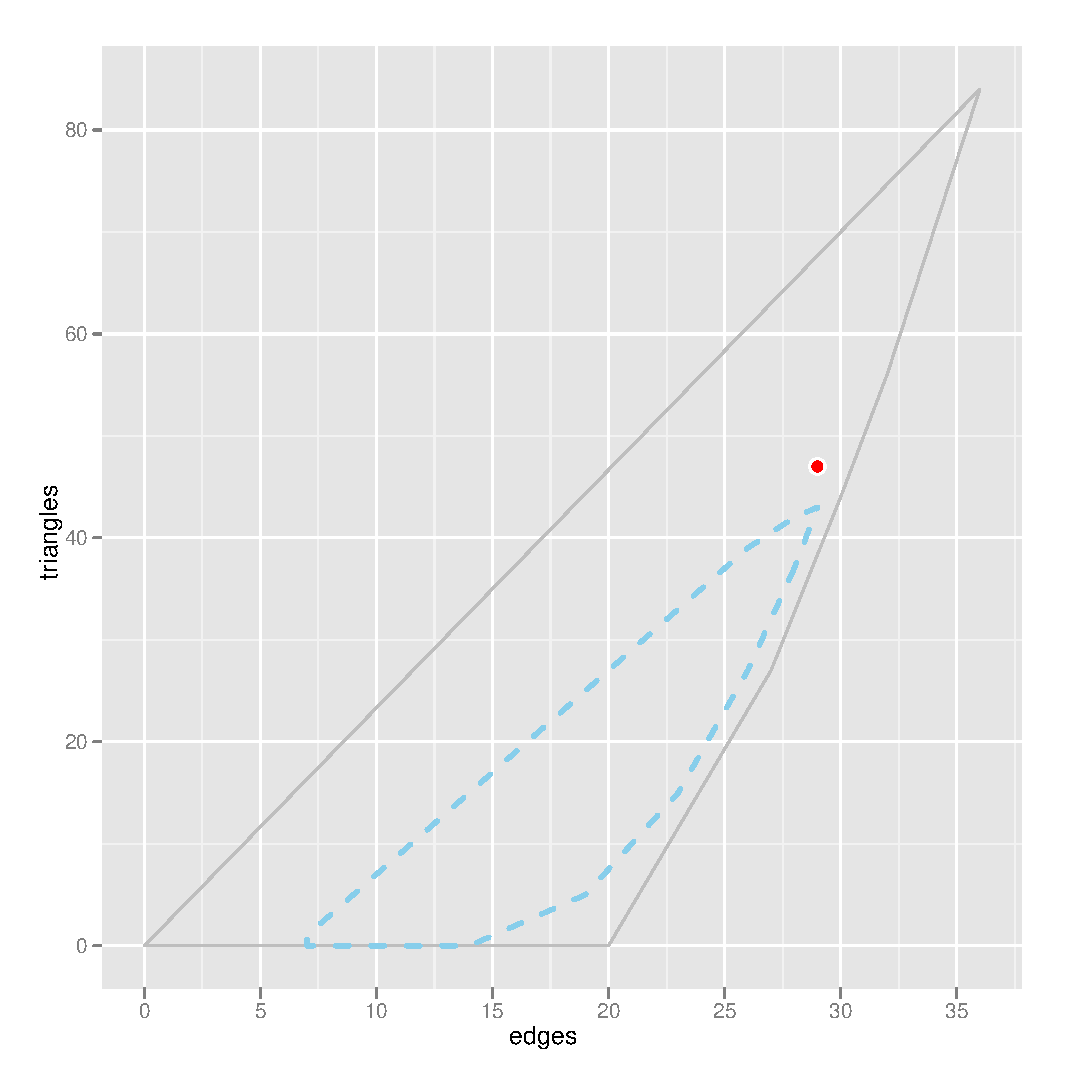
\includegraphics[height=2.8in,width=2.8in]{Figures/MCsample-far}
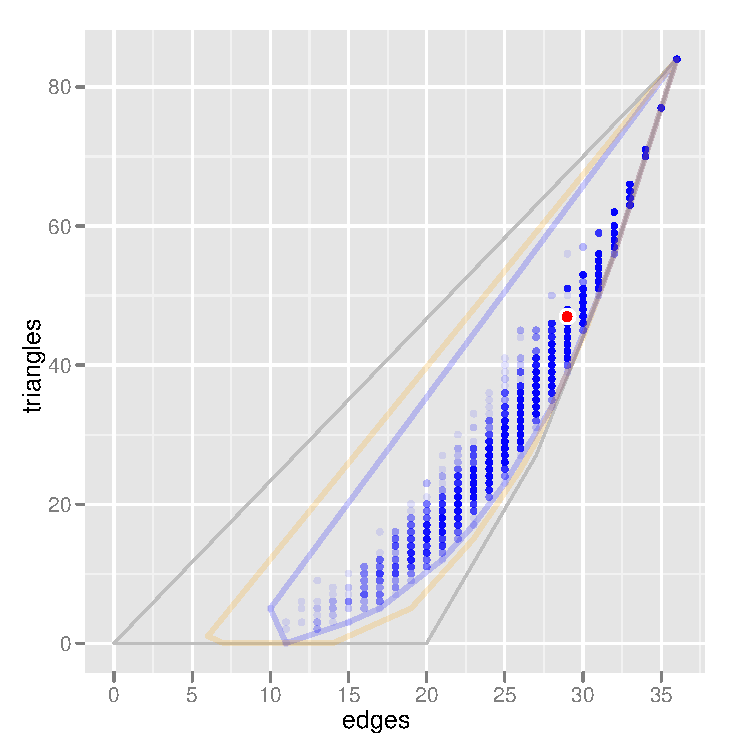
\includegraphics[height=2.8in,width=2.8in]{Figures/MCsample-MLE}
\caption{The network statistics for 10,000 Monte Carlo samples generated from models 
with the natural parameter $\eta$ set to $(0,0)$ (top) and the MLE, $(-0.389, 0.418)$ 
(bottom).  The observed data has network statistics of $(29,47)$, depicted by the 
larger point with white outline.  When $\eta$ is the MLE, the observed statistic is 
exactly the mean of the MC sample points generated from the model with this parameter 
value. }
\label{F:MC cloud}
% (-0.3890151, 0.4177752)
\end{figure}
For this problem, the MLE for $\eta$ is found to be
\begin{align*}
\etaMLE = (-0.389, 0.418).
\end{align*}

\subsubsection{Case: MLE does not exist; observed statistic on one-dimensional face}
If the observed data has network statistic $(31,50)$ and lies on the 
boundary of the convex support as depicted in Figure \ref{F:MC face}, the MLE does not 
exist.  To be precise, the observed network statistic $(31,50)$ lies on the interior 
of a line segment on the boundary with end points $(30,44)$ and $(32,56)$. 
Our algorithm begins as before, generating MC�sample point clouds to explore the 
sample space, as depicted in Figure \ref{F:MC face}.  Because the sail-shaped convex 
support is not known, the algorithm cannot determine at the outset  that the MLE does 
not exist; it can only generate more sample point clouds as it climbs the log 
likelihood surface, with successive clouds moving towards the observed statistic.
Eventually, the observed statistic will lie exactly on the boundary of a sample cloud.  
When this occurs, the algorithm must 
\begin{enumerate}
\item determine empirically the face, $F$, on which the observed statistic lies in the 
relative interior of,
\item decide if $F$ is in fact the boundary of the convex support $C$.
\end{enumerate}  

The first task can be done using the linear programming functions provided to us in 
the \texttt{rcdd} package.  The second task turns out to be very difficult to do.  
For now, we assume that if a substantial portion of the sample points generated, say 
60\%, land on this empirically determined face $F$, then it is in fact a boundary of 
the convex support $C$.  


In this example, the algorithm has determined empirically that $(30,44)$, $(31,50)$, 
and $(32,56)$ lie on a one-dimensional face, as depicted in Figure \ref{F:MC face} 
(bottom).  If less than 60\% of the sample points land on this empirical face, the 
algorithm continues to sample, trying to get a sample point cloud even closer to the 
observed statistic.  We choose such a high proportion for a cut off to eliminate---or 
at least, greatly reduce---the possibility of misidentifying a boundary.
(We deal later with a case where 100\% of the MC sample points form a face which is 
\emph{not} on the boundary of $C$.)
\begin{figure}[!ht]
\centering
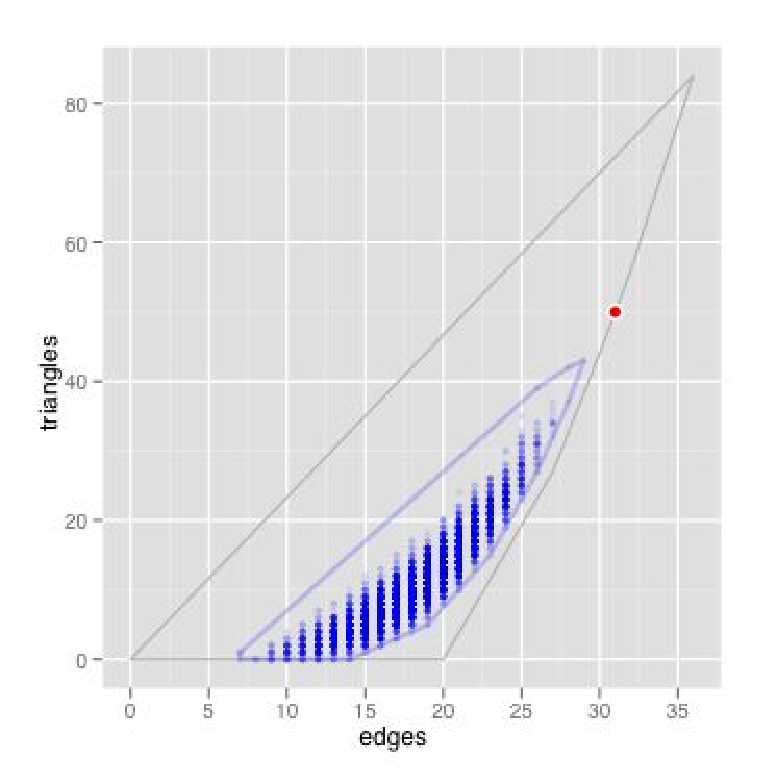
\includegraphics[height=2.7in,width=2.7in]{Figures/MCsample-boundary}
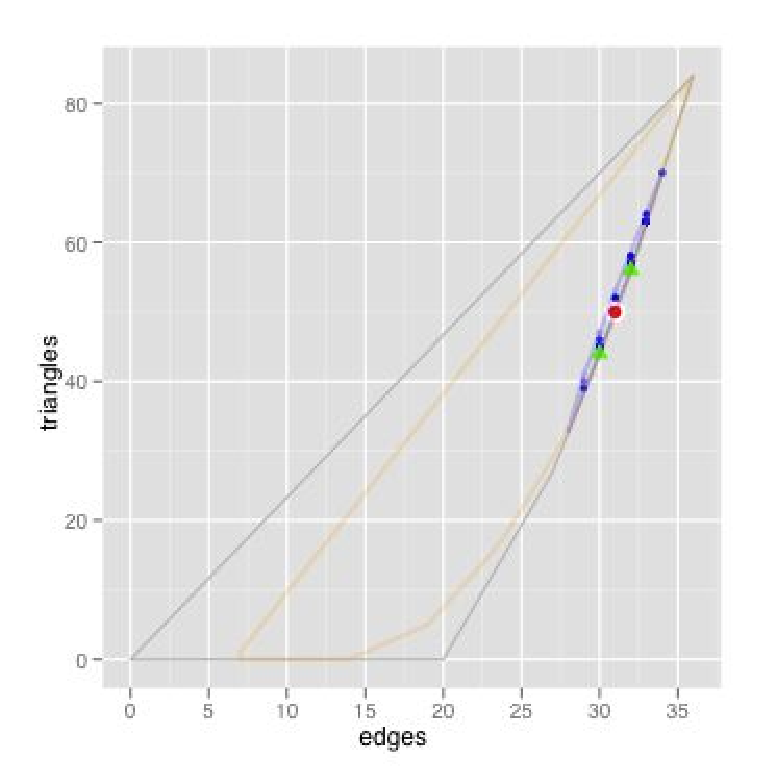
\includegraphics[height=2.7in,width=2.7in]{Figures/MCsample-77face}
\caption{The network statistics for 10,000 Monte Carlo samples for the model with 
observed network statistic $(31,50)$, depicted by the larger point with white 
outline, lying on the boundary of the convex support (top).
In the bottom figure, the algorithm has identified a face defined by $(30,44)$, 
$(31,50)$, and $(32,56)$, marked by triangles in the figure (the triangle for 
$(31,50)$ is not visible since it is the observed statistic).  
Here, 77\% of the MC sample points fall on these three points.  The 
lighter colored polytope is the convex hull of all previously sampled points.
}
\label{F:MC face}
\end{figure}

By identifying the empirical face $F$ on whose interior the observed statistic lies, 
the algorithm has not only concluded that the MLE does not exist in the conventional 
sense, it has also defined $F$ as the convex support for the new limiting conditional 
model, which is also an exponential family.  

The algorithm proceeds to maximize this new exponential family using the same 
iterative approach as before.  The gradient of the LCM log likelihood is approximated 
using \eqref{E:nabla ell approx LCM},
\begin{align*}
	\nabla \ell( \eta )^{LCM} \approx g(\yobs) - \frac{1}{k} \sum_{i=1}^k g(Y_{(k)})
\end{align*}
where $g(Y_{(1)}), \ldots, g(Y_{(k)})$ is the subsample of the MC sample points 
restricted to the empirical face: $(30,44)$, $(31,50)$, and $(32,56)$ in this case.  
The maximizer of this log likelihood, $\etaLCM$, is found to be
\begin{align*}
\etaLCM = (120.9, -20.1).
%(120.91090 -20.12784)
\end{align*}
The LCM, however, is not identifiable, since the support is now only one-dimensional 
compared to two in the original model (EXPLAIN BETTER).  
That is, there must exist a constancy space of this new model, $\Gammalim$, such that 
\begin{align} \label{E:Gammalim}
\ell( \eta + \gamma )^{LCM} = \ell( \eta )^{LCM}
\end{align}
for any $\gamma \in \Gammalim$.

The empirical face $F$ and the observed statistic also define a normal cone, which in this case is a single direction, 
\begin{align*}
	\delta = (6,-1),
\end{align*}
which is called a generic direction of recession (GDOR).  Exponential family theory 
states that the log likelihood is a strictly concave function of $\eta$.  For a 
maximizer to exist then, there must be a direction along which the log likelihood 
function increases to $+\infty$.  This direction is exactly the $\delta$ found above, 
and combined with a specific point in the natural parameter space, $\etaLCM$, 
\begin{align} \label{E:GDOR lim}
	\lim_{s \to +\infty} \ell( \etaLCM + s \delta) = \sup_{\eta} \ell(\eta),
\end{align}
where  $\ell(\cdot)$ is the log likelihood of our original model.

The GDOR, $\delta$, of the original model is also a direction of constancy the new 
model.  
Then by \eqref{E:Gammalim} and \eqref{E:GDOR lim}, note that $\ell(\etaLCM + \gamma + 
s \delta)$ goes off to $+\infty$ as $s$ increases.  
In order to construct a one-sided confidence intervals, we need to find the value of 
$s$ for which the probability that the distribution allocates to the event that a 
sample falls on the face of interest is 5\%, that is,
\begin{align*}
P_{\etaLCM + \gamma + s \delta}(g(Y) \in F ) = 0.05.
\end{align*}
Although we cannot evaluate the probability function above, we can generate MC samples 
of $g(Y_1), \ldots, g(Y_m)$ from the distribution with parameter $\etaLCM + \gamma + s 
\delta$ and see for what value of $s$, 5\% of the sample lies in the empirical face we 
found.  

Some numerical work shows that for $\eta = (9.19, -1.51)$, we get 5\% of the MC sample 
on this face.  Or, in terms of non-simultaneous 95\% confidence intervals for the 
components of $\eta$,
\begin{align*}
	[9.19, +\infty)\\
	(-\infty, -1.51],
\end{align*}
where the direction of the interval for the second component is flipped because the 
second component of $\delta$ is negative.

\textbf{Mean value parameters? Are they any more interpretable here?  nice pictures}

%Because our sample space for graphs is still manageable at 69 billion points, we can 
%in fact use numerical optimization methods like trust (CITE?) on the original log 
%likelihood, passing in first and second derivative functions.  Depending on the 
%settings for tolerance, we can get a trust routine to return to what it thinks is an 
%MLE,  
%\begin{align*}
% 	\hat{\eta}_{\textrm{trust}} = (135.6, -22.6),
% \end{align*}
%which are well within our confidence intervals.

%%%%%%%%%%%%%%%%%%%%%%%%%%%%%%%%%%%%%%%%%%%%%%%%%%%%%
\subsubsection{Case: MLE does not exist; observed statistic on zero-dimensional face}
If the observed data has network statistic $(27, 27)$, the point is an extreme point 
of the convex support $C$ (it is a square point on the boundary of the sail in Figure~
\ref{F:g9-hull}) and the MLE does not exist.  In this case, the point itself is the 
face with zero-dimension.  The algorithm proceeds as before, and concludes that the 
point $(27,27)$ is the empirical face $F$ and on the boundary of the hull.
In this case, the limiting conditioning model is completely unidentifiable, and thus 
any value for $\eta$ will be a maximizer.  Our particular implementation found that
\begin{align*}
	\etaLCM = (94.0, -20.4 ).
\end{align*}
The normal cone to the observed statistic in this case is two-dimensional, bounded by 
two vectors,
\begin{align*}
	 \{ (3.857,   -1),	(5.667,   -1) \}.
\end{align*}
If we choose the average of these two vectors, $\delta = (4.76, -1)$, and proceed as 
before, then we find 95\% one-sided confidence intervals for $\eta$ of 
\begin{align*}
%14.495152 -3.703202 
	[14.5, +\infty)\\
	(-\infty, -3.7],
\end{align*}

\textbf{MEAN VALUE PARAMETERS?}


%%%%%%%%%%%%%%%%%%%%%%%%%%%%%%%%%%%%%%%%%%%%%%%%%%%%%
\subsubsection{Case: MLE exists but observed statistic is very near boundary}
If the observed data has network statistic $(21, 4)$, it is in fact on the interior of 
the convex support and so the MLE exists.  
The approaches of \citet{Handcock:degeneracy} and \citet{Rinaldo:2009} would have 
noted that from a mean value pararmeter perspective, this observed statistic likely 
corresponds to a degenerate distribution. The Shannon entropy function would show this 
point to have extremely small entropy, corresponding to a model that puts most of its 
probability on very few points.

The log likelihood for this model is extremely flat, causing some disagreement among 
numerical optimization routines for MLE estimates, though log likelihood values are nearly 
identical.  Using a trust optimization routine we calculate that 
\begin{align*}
%$(24.44, ?6.65)$ from optim.
\etaMLE = (28.86, -7.76).
\end{align*}
The most problematic aspect of this model for us here, however, is that our algorithm 
concludes---incorrectly, of course---that the MLE does not exist, and proceeds to 
calculate the MLE of an LCM.

How does this happen?

Our algorithm begins in the same manner as described previously.  As the algorithm 
proceeds uphill on the log likelihood function, it will iterate $\eta_k$ to a value 
(for example, $(35.34, -9.56)$) where all 10,000 MC sample points generated from the 
model with this parameter value fall on the six points on the line segment between 
$(20,0)$ and $(25,5)$, as depicted in Figure~\ref{F:MC problem}.  The observed value $
(21,4)$ is one of these six points.
In order for the algorithm to have correctly identified the boundary here and conclude 
that $(21,4)$ was on the interior, the extreme point $(27,27)$ would need to have 
occurred in the MC sample.  However, for the parameter value that we consider, model 
assigns a probability of 0.000032 to this point.  Even the MLE model only assigns a 
probability of about 0.00045 to this point.  So, the extreme point that is critical 
for fully determining the convex support is in fact assigned very low probability by 
the MLE model.

\begin{figure}[!h]
\centering
%%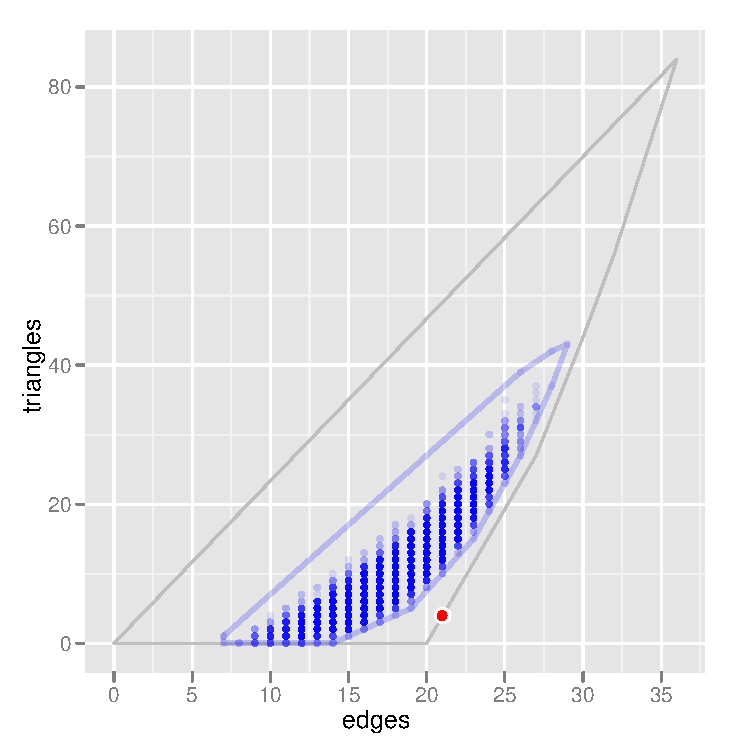
\includegraphics[height=2.4in,width=2.4in]{Figures/MCsample-problem}
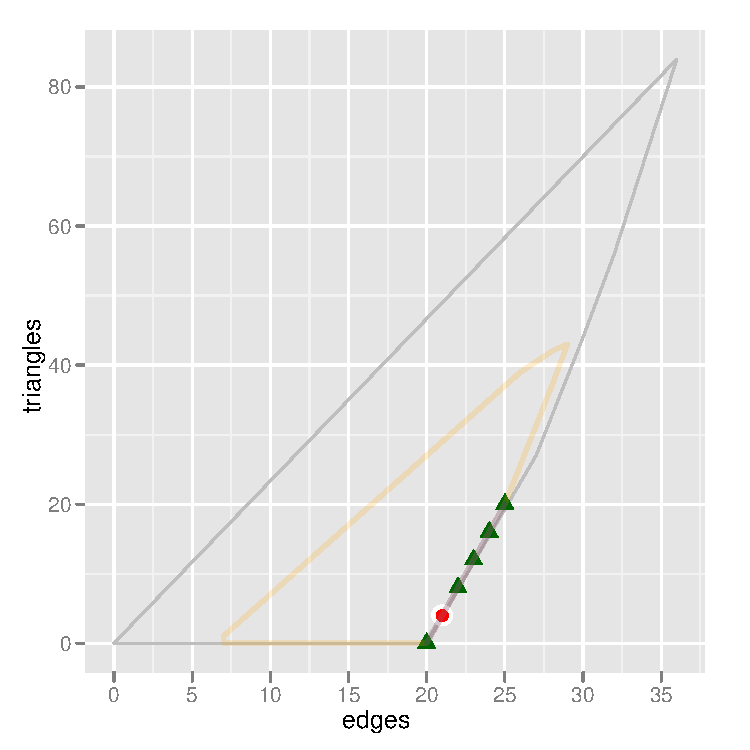
\includegraphics[height=4.5in,width=4.5in]{Figures/MCsample-fakeface}
\caption{An observed statistic at $(21,4)$, in the interior of the convex hull but 
close to the boundary.  It is quite feasible to generate 10,000 MC 
samples where all 10,000 points lie on a line that appear to be a one-dimensional 
face, marked by the 
triangles in the figure above.  The lighter colored polytope is the convex hull of all 
previously 
sampled points used to derive this empirical face.}
\label{F:MC problem}
\end{figure}

According to the algorithm, this line segment is a boundary of the convex support on 
which the observed statistic lies on the interior of, and the MLE does not exist.  It 
proceeds as in the first example, and seeks to find the MLE of the LCM,
\begin{align*}
	\etaLCM = (35.38, -9.39),
\end{align*}
and then calculates one-sided confidence intervals for $\eta$.

On first glance this is very troubling: our algorithm arrives at the wrong conclusion 
about the existence of the MLE, and $(35.38, -9.39)$ does not look particularly close 
to the true MLE of $(28.86, -7.76)$.  However, we believe a step back needs to be 
taken and the goal of the analysis reconsidered.  What was the purpose in finding the 
MLE?  In particular, what does one do with these numbers once they are found?

If the end goal is to try to interpret meaning out of these numbers by their sign and  
magnitude (\textbf{a questionable approach?  or at least dangerous?}), then we indeed 
have a problem---our numbers are just wrong.  However, if the MLE is viewed as an 
index into a specific model that assigns the highest probability to the observed data,
then we claim that the model we have found---the LCM with parameter value $\etaLCM$---
is in fact remarkably similar to the original model indexed by the true MLE.  A 
reasonable metric for this comparison is a sum of the absolute difference in 
probabilities assigned to each point in the sample space,
\begin{align*}
	\sum_{y \in \YY} \abs{ P_{\etaMLE}(g(Y) =g(y) ) -  P_{\etaLCM}(g(Y) = g(y))  }.
\end{align*}
The probabilities assigned by each of these models to the six points on the 
empirically determined face is summarized in Table~\ref{T:LCMvsMLE}.

% latex table generated in R 2.11.1 by xtable 1.5-6 package
% Fri Sep 10 13:22:25 2010
\begin{table}[h!] \label{T:LCMvsMLE}
\begin{center}
\caption{Probabilities assigned by LCM model with parameter value $\etaLCM$ and 
original model with parameter value $\etaMLE$ to six points on empirical face.  The 
observed statistic is $(21,4)$.}

\begin{tabular}{rrrrr}
\\  \hline
 & Edges & Triangles & LCM & MLE \\ 
  \hline
1 & 20 & 0 & 0.3414 & 0.3425 \\ 
  2 & 22 & 8 & 0.2019 & 0.2009 \\ 
  3 & 21 & 4 & 0.3914 & 0.3911 \\ 
  4 & 23 & 12 & 0.0566 & 0.0561 \\ 
  5 & 24 & 16 & 0.0081 & 0.0080 \\ 
  6 & 25 & 20 & 0.0005 & 0.0005 \\ 
   \hline
   &  &  & 1.0000 & 0.9990 \\ 
\end{tabular}
\end{center}
\end{table}

Here, the sum of the absolute value of differences on these empirical points is only 
$0.0031$.  Including the additional 0.001 of probability on points that are outside 
the LCM support, this total still only comes to $0.0041$, a difference that would seem 
insignificant for most applications.  

Of course, there may be practical issues: a researcher may want software to simply 
return MLE values to keep around for later analysis.  Here, we are suggesting the 
analysis return LCM MLE values and an LCM model (perhaps in the form of the convex 
support).  The researcher may understandably be confused, especially if he knew in 
advance that the MLE was guaranteed to exist.  However, any analysis (other than the 
parameter value magnitude study) would still work as before, though perhaps not ``out 
of the box".

It may be of interest to note that $\etaLCM$ and $\etaMLE$ index nearly identical 
models in the LCM, with the difference due almost entirely to the lack of 
identifiability of the LCM.  A normal direction to the empirical face is $\delta = 
(4,-1)$, which is a direction of constancy for the LCM (that is, $\delta \in \Gammalim
$).  Then by \eqref{E:Gammalim}, 
\begin{align*}
	\ell(\etaLCM)^{LCM} &= \ell( \etaLCM + \gamma )^{LCM}\\
				 &= 	\ell(\etaLCM + k \, (4,-1))^{LCM}.
\end{align*}
If we had perfect knowledge and chose $k = -1.63$,
\begin{align*}
	\etaLCM  -1.63 \, (4,-1)= (28.86, -7.76) 
\end{align*}
matching the MLE to the significant figures considered.  Thus in this case, $\etaLCM$ 
and $\etaMLE$ index nearly identical models of the LCM.

If we finished the analysis as before and computed one-sided 95\% confidence intervals 
for $\eta$, we get 
\begin{align*}
%14.495152 -3.703202 
	[20.46, +\infty)\\
	(-\infty, -4.85].
\end{align*}
%20.462923 -4.850603 

%\begin{align*}
%	\hat{\theta}_{MLE} &= (28.85685, -7.75672)\\
%	\hat{\theta}_{LCM} &= (35.3831787, -9.387266),
%\end{align*}

%Well, remember that for LCM's we are looking to construct one-sided CIs.  But here, 
%what happens if we go off to infinity in this supposed direction of recession?  The 
%log-likelihood will eventually dip back down!  So, we can constructed two-sided CI's, 
%I think.  But, my calculations got me something that seems pointlessly wide: 
%\begin{align*}
% (3.503179,  -1.417266 )\\
% (71.22318,  -18.34727 ).
%\end{align*}

%%%%%%%%%%%%%%%%%%%%%%%%%%%%%%%%%%%%%%%%%%%%%%%%%%%%%


\subsection{Three-dimensional sufficient statistic}

In order to increase the complexity of the problem yet still have the ``truth" for 
comparison, we also considered 7-node graph with network statistics edges, two-stars, 
and triangles, a classic model in the literature first suggested by \citet{Frank:
1986}.  Since then it has been criticized for its problematic behavior by \citet
[really? check this]{GOF}, precisely related to the issue of non-existence MLEs (or 
degeneracy???).

The algorithm proceeds in exactly the same way, the difference now being that the 
empirical face may have as many as two dimensions instead of one.  This makes for a 
more interesting variety of constancy spaces for the LCM.  We only consider cases here 
that add a notably different flavor than the two-dimensional case.

\subsubsection{Observed value, $y_{obs}$, is on two-dimensional face}
\subsubsection{Observed value, $y_{obs}$, is on one-dimensional face}
\subsubsection{MLE does not exist; observed statistic on two-dimensional face but not 
fully discoverd}

Set $y_{obs} = (14, 8, 43).$
This point is on the boundary, which is a 2-dim face.

The MC sample, however, does not cover the entire face.  This is a new scenario, but 
it should not be a problem.  Those points on the actual face that are not included are 
simply points of low probability.

Only issue outstanding with this is how long it takes to find the LCM MLE.  Having a 
surprisingly hard time with this.  Question: is it doing any worse than when we 
started with a 2-dim sample space?

\section{Example: \textit{e. coli}?}
\section{Example: Faux Magnolia High School?}
\citet{advancesp*,statnet-tutorial} utilize a adolescent friendship network data set 
of 1,461 students in grade 7--12 derived from the National Longitudinal Study of 
Adolescent Health.  The data set, which \citeauthor{statnet-tutorial} refer to as Faux 
Magnolia High School, is a model-based simulation from the original data set, where 
the simulation is necessitated to maintain confidentiality.
